Die folgenden Abbildung \ref{img:pruefaufbau} zeigt eine Skizze des verwendeten Prüfaufbaus.
Zur Vereinfachung wird die Skizze ohne Halterungen erstellt.

\begin{figure}[H]
	\centering
	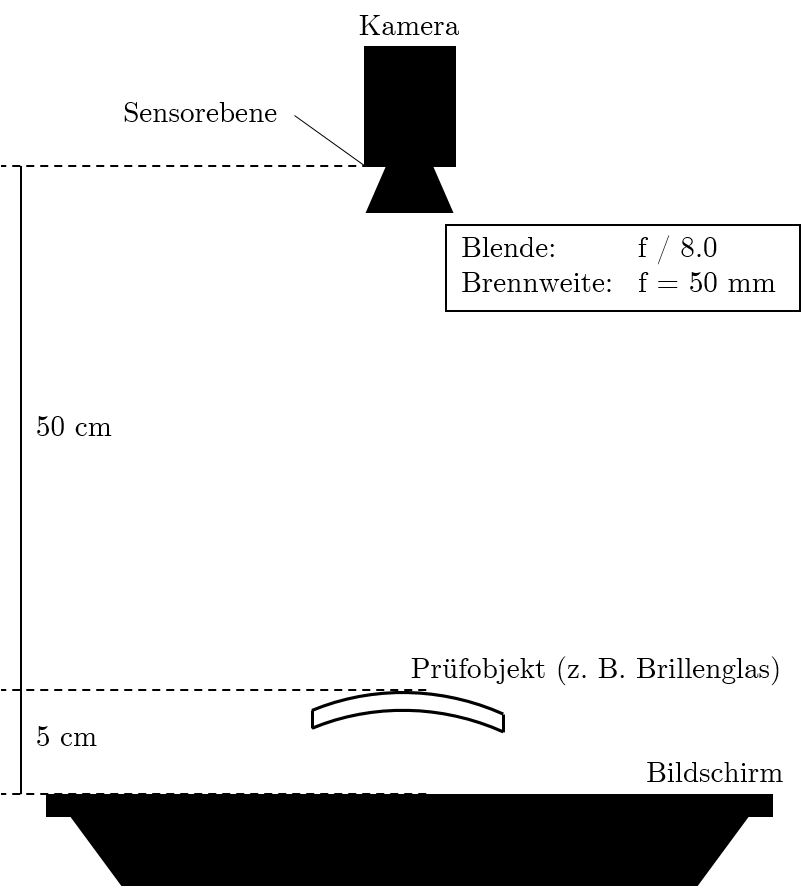
\includegraphics[width=0.5\textwidth]{03_sichtpruefungDurchLichtstreuung/pruefaufbau/figures/aufbau}
	\caption[Prüfaufbau]{Prüfaufbau (Abbildung nicht maßstabsgetreu)}
	\label{img:pruefaufbau}
\end{figure}

\noindent
Die Parameter des Prüfaufbaus wie z. B. Kameraeinstellungen und Entfernungen lassen sich aus Abbildung \ref{img:pruefaufbau} entnehmen.
Es gilt zu beachten, dass die Entfernung zur Kamera nicht am Objektiv, sondern an der Sensorebene gemessen wird.
Der Grund liegt darin, dass Objektive unterschiedliche Größen haben, weshalb die Entfernung andernfalls für verschiedene Objektive unterschiedlich sein würde.
Die Sensorebene einer Kamera ist die Position des Kamerasensors, an der das einfallende Licht aufgenommen wird.
Dieser Aufbau wird zur Erzeugung von Bildmaterial für diesen Projektbericht verwendet.
Zur Auswertung und Verknüpfung des Bildmaterials wird die NeuroCheck-Software eingesetzt.
Die Prüfobjekte sind transparente Brillengläser mit Eingravierungen und einzelnen Fehlstellen.